شبکه عصبی مورد استفاده در هر سه مقاله، شبکه عصبی پیچشی \پانویس{Convolutional neural network} می‌باشد. این نوع شبکه های عصبی از لایه های مختلفی تشکیل شده اند که هر کدام از آنها ویژگی های منحصر به فردی از داده ورودی را تشخیص می‌دهند، سپس از مقایسه ویژگی های بدست آمده با الگوهای از پیش یاد گرفته شده احتمال تعلق داده ورودی به دسته های مختلف خروجی بررسی می‌شود. بسته به نوع قرار گرفتن لایه ها در کنار هم معماری های مختلفی به وجود خواهد آمد. در ادامه به بررسی معماری شبکه های عصبی هر مقاله به صورت جداگانه می‌پردازیم.

\زیرقسمت {شبکه عصبی \آ}
داده های ورودی به شبکه عصبی این مقاله به صورت آرایه های دوبعدی (سیگنال زمانی * کانال) می‌باشد. در این مقاله بسته به نوع لایه های پیچشی، سه سناریویی مختلف برای معماری شبکه عصبی بیان می‌شود. در حالت اول عملیات پیچش فقط در راستای زمان، در حالت دوم عملیات پیچشی در راستای کانال و در حالت سوم  عملیات پیچش هم در راستای زمان و هم در راستای کانال بکار برده می‌شود. شبکه عصبی پیاده سازی شده در این پروژه برای \آ\ حالت اول می‌باشد که شماتیک کلی آن در شکل \رجوع{cnn1} قابل مشاهده می‌باشد.

\begin{figure}
\centering
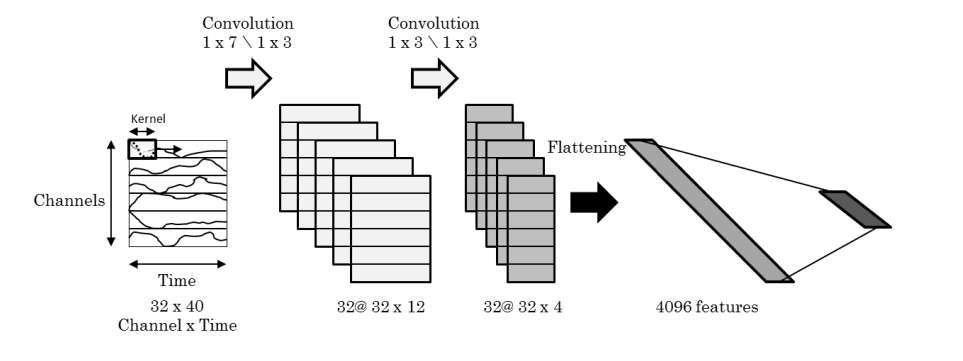
\includegraphics[width=15cm]{img/cnn1.png}
\شرح{شبکهٔ عصبی \آ\ \مرجع{Sakhavi2018}}
\برچسب{cnn1}
\end{figure}

به طور خلاصه در این معماری،‌ ابتدا از یک لایه پیچشی ۳۲ تایی با ابعاد کرنل (۷*۱) و لغزش (۳*۱) سپس لایه پیچشی ۳۲ تایی دیگر با ابعاد کرنل (۳*۱)و لغزش (۳*۱) استفاده شده است. خروجی این دو لایه بعد از یکپارچه سازی به لایه کاملا همبند\پانویس{Fully connected} وارد می‌شود و در نهایت از لایه خروجی \مل{Softmax} جهت کلاس بندی استفاده می‌شود. توابع فعال سازی لایه ها از نوع \مل{Relu} بوده و همچین برای جلوگیری از پدیده بیش برازش از حذف تصادفی \پانویس{Drop-out} بعد از توابع فعال سازی استفاده شده است. 

\زیرقسمت {شبکه عصبی \ب}
معماری شبکه عصبی بکار برده شده در این مقاله در تعداد ورودی با دو مقاله دیگر متفاوت است. با توجه مطالب بیان شده در بخش پیش پردازش، داده های ورودی این شبکه عصبی ۲۰ آرایه دوبعدی با ابعاد(۲۸*۲۸) می‌باشد.  بنابراین به نوعی می توان گفت  این شبکه عصبی ۲۰ ورودی دارد. هر کدام از این ورودی ها پس از عبور از سه لایه پیچشی در نهایت با هم ادغام می‌شوند و  پس از عبور از لایه کاملا همبند و لایه خروجی کلاس بندی خواهند شد. شماتیکی از معماری این شبکه عصبی در شکل \رجوع{cnn2} قابل مشاهده می‌باشد. 

\begin{figure}
\centering
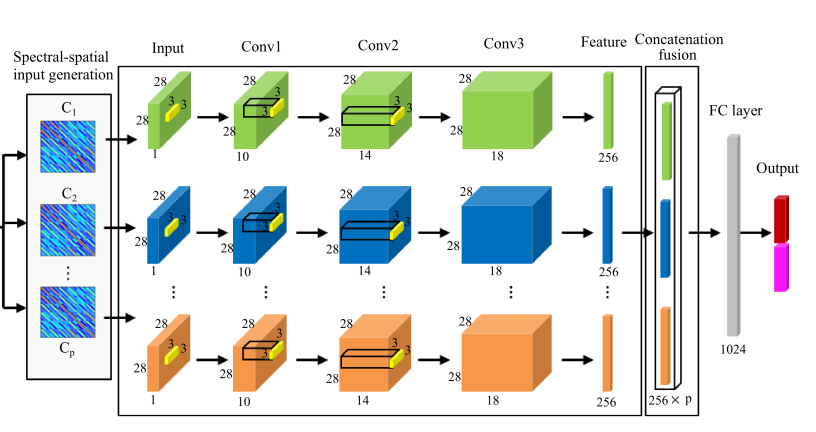
\includegraphics[width=15cm]{img/cnn2.png}
\شرح{شبکهٔ عصبی \ب\ \مرجع{Kwon2020}}
\برچسب{cnn2}
\end{figure}

\زیرقسمت {شبکه عصبی \پ}
هدف این مقاله دسته بندی سیگنال های مربوط به زاویه چرخش ۰، ۹۰ و ۱۸۰ درجه می‌باشد. در این مقاله با استفاده از ادغام نتایج دو شبکه عصبی این دسته بندی صورت می‌گیرد. شبکه عصبی اول با هدف تشخیص آنکه حرکتی صورت گرفته است یا خیر و شبکه عصبی دوم با هدف تشخیص زاویه چرخش طراحی شده اند. شماتیکی از این شبکه عصبی و لایه های بکار برده شده، در شکل \رجوع{cnn3} قابل مشاهده می باشد.

\begin{figure}
\centering
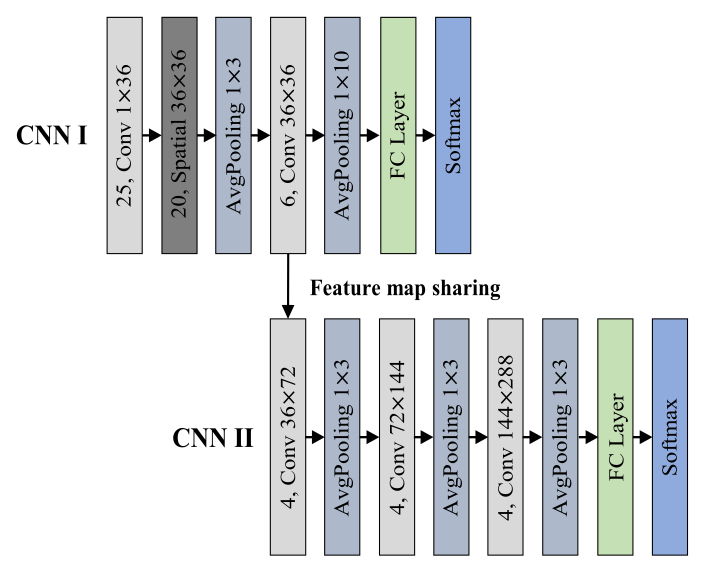
\includegraphics[width=12cm]{img/cnn3.png}
\شرح{شبکهٔ عصبی \پ\ \مرجع{Jeong2020}}
\برچسب{cnn3}
\end{figure}

اما همانطور که بیان شد، در این پروژه از این شبکه عصبی برای دسته بندی داده های مربوط به مقاله اول استفاده شد و از آنجایی که داده های مقاله اول فقط مربوط سیگنال های حرکتی بوده بنابراین فقط بخش دوم این شبکه عصبی پیاده سازی شد.
